\documentclass[12pt, a4paper]{article}
\usepackage[utf8]{inputenc}
\usepackage{amsmath}
\usepackage{amsfonts}
\usepackage{amsthm}
\usepackage{array}
\usepackage{graphicx}
\usepackage{parskip}
\usepackage[pdfencoding=auto]{hyperref}
\usepackage{fancyhdr}
\usepackage{lastpage}
\usepackage{tikz}
\usepackage{float}
\usepackage{listings}
\usepackage{color}
\usepackage{caption}
\usepackage{authblk}
\usepackage{longtable}
\usepackage[acronym]{glossaries}
\usepackage[nottoc]{tocbibind}
\usepackage[cache=false]{minted}
\usemintedstyle{default}
\newminted{haskell}{frame=lines,framerule=2pt}
\newminted{R}{frame=lines,framerule=2pt}
\graphicspath{{./images/}}

\tikzstyle{bag} = [align=center]

\title{%
      Analysis of Software Design Principles \\
      under Complex Network Theory\\
}
\author{Juan Pablo Royo Sales \& Francesc Roy Campderrós}
\affil{Universitat Politècnica de Catalunya}
\date\today

\pagestyle{fancy}
\fancyhf{}
\fancyhead[C]{}
\fancyhead[R]{UPC MIRI}
\fancyhead[L]{CSN - Final Work}
\fancyfoot[L,C]{}
\fancyfoot[R]{Page \thepage{} of \pageref{LastPage}}
\setlength{\headheight}{15pt}
\renewcommand{\headrulewidth}{0.4pt}
\renewcommand{\footrulewidth}{0.4pt}

\newacronym{netdyn}{Network Dynamics}{Network Dynamics}
\newacronym{degdist}{Degree Distribution}{Degree Distribution}
\newacronym{growdeg}{Time Growth Degree}{Growth of Vertex Degree over time}
\newacronym{prefatt}{G Pref Attachment}{Growth + Preferential Attachment}
\newacronym{randatt}{G Random Attachment}{Growth + Random Attachment}
\newacronym{nprefatt}{NG Pref Attachment}{No Growth + Preferential Attachment}
\newacronym{baral}{Barabasi-Albert model}{Barabasi-Albert model}
\newacronym{indegree}{Incomming Degree}{Incomming Degree Language Set}
\newacronym{zeta}{Zeta}{Zeta Model}
\newacronym{aic}{Akaike}{Akaike Information Criterion}
\newacronym{dispp}{Displaced Poisson}{Displaced Poisson Model}
\newacronym{dispg}{Displaced Geometric}{Displaced Geometric Model}
\newacronym{hc}{High Cohesion}{High Cohesion}
\newacronym{lc}{Low Coupling}{Low Coupling}
\newacronym{cnt}{Complex Network Theory}{Complex Network Theory}
\newacronym{fp}{Functional Programming}{Functional Programming}
\newacronym{oop}{Object Oriented Programming}{Object Oriented Programming}
\newacronym{loc}{LoC}{Lines of Code}
\newacronym{cdg}{CDG}{Call Dependency Graph}
\newacronym{fu}{FU}{Functional Units}

\newtheorem{hyp}{Hypothesis}

\begin{document}

\maketitle

\tableofcontents

\section{Introduction}
One of the most well known Software Design principles in \textbf{Software Engineering} is \acrfull{hc} and \acrfull{lc}, which is well described here~\cite{cohesion_coupling}.

As this two principles states a \textit{robust Software} should be design with \acrlong{lc} between their modules and \acrlong{hc} inside it. 

In other words, a Software that fullfil this characteristics should be very connected in their minimum \acrfull{fu} (Functions inside same file, Methods inside a class, etc), and with few connections between their coarse grained \acrshort{fu} (a.k.a Modules or Packages).

In this work, we are going to formulate some hypothesis which we believe it can been empirically proved and shown the relationship between these principles and how to measure them with \textbf{\acrfull{cnt}}.
At the same time, we are going to analysis different kinds of software of different sizes and build under different language paradigms to see if the tool set that \acrshort{cnt} provides are suitable for the general case. 

\section{Preliminaries}
In this section we are going to describe how and why the different Language Paradigms are selected and what is the criterion for selection of different Software solutions to be evaluated.

On the other hand as well, we are going to formulate some hypothesis that are going to guide our work to see if our assumptions can empirically been proved using \acrlong{cnt}.

\subsection{Context}
We have selected the most important $2$ main Language Paradigm to conduct the analysis: \acrfull{fp} and \acrfull{oop}. 

The reasons behind this decision are basically the following:

\begin{itemize}
    \item \textbf{95\%} of Software in the Industry are built with one of these 2 Paradigms according to the last results of this well-known survey~\cite{so_survey}.
    \item Due to the intrinsic nature of each of those Paradigms we have some hypothesis that we are going to describe later that can lead to different conclusion and Metrics
    \item If we can deduce some Software Design properties analyzing these 2 Paradigms we can generalize for the rest because they are quite different in nature and covers almost the whole Industry.
    \item We also believe that Software Principles should apply indistinguishably the Paradigm. 
\end{itemize}

On the other hand the selection of the programs to be analyzed are the following:

\begin{itemize}
    \item Most of the software are Open Source or Free software that can be download publicly either from~\cite{github} or from~\cite{maven_repo}.
    \item Software that are marked as \textbf{PRIVATE} are Big Projects from Privates Companies that don't want to reveal the Sources Code and Names for Commercial reasons.
    \item In the case of \textbf{PRIVATE} \acrshort{fp} Solution, it belongs to a Company one of the authors of the current work is working right now.
    \item In the case of \textbf{PRIVATE} \acrshort{oop} Solution, it belongs to a Company one of the authors of the current work worked in the past.
    \item In both cases, taken anonymous data for conducting this analysis has been agreed with legal representatives of those Companies.
\end{itemize}

On the last hand we are going to use \textit{Haskell} Programs for analyzing \acrlong{fp} and \textit{Java} Programs for \acrlong{oop}. We believe that right now both are the most representative
ones in their Paradigm fields.

\subsection{Hypothesis}
In this work we are trying to prove the following \textbf{Hypothesis} that we consider can be proved using \acrfull{cnt}.

\begin{hyp}
Given any Software Program Solution, its Network Metrics should be between the  $1$st Quartile and $3$rd Quartile, according to the average of the Network Metrics that we have been identified in this work,
to be considered as a well Software Designed Solution.
\end{hyp}

\begin{hyp}
Any \acrlong{oop} Program have a better modularity in terms of \acrlong{cnt} Metric rather than \acrlong{fp} Programs.
\end{hyp}

\begin{hyp}
The more \acrfull{loc} a Program have, the better Modularity it presents.
\end{hyp}
    
\begin{hyp}
If the Software follows the principle design of \acrshort{hc} and \acrshort{lc}, the \acrfull{degdist} of the Generated Graph should follow a power-law like.
\end{hyp}

\section{Results}
In this section first we are going to describe the \textbf{Experiments} conducted and after that we have obtained after running the different experiments; this is what we call \textbf{Metrics} subsection.

\subsection{Experiments}
In this section we are going to described how the experiment have been set up in order to prepare the graphs for taking the desired metrics, that could allow us to explain and verify the proposed hypothesis.

\subsubsection{Preliminaries}
In order to determine if a Software fullfil the 2 Software Design Principles that we want to analyze, \acrshort{hc} and \acrshort{lc}, 
we need to extract the \acrfull{cdg} from the programs that we want to analyze.

In \acrshort{cdg}, \textbf{nodes} are \acrlong{fu}: \textit{Functions} in the case of \acrshort{fp} and \textit{Methods} in the case of \acrshort{oop}.
An \textbf{edge} is when from inside a \acrshort{fu} another \acrshort{fu} is called or invoked.

Therefore, we need to build this \acrlong{cdg} in order to establish how the different Modules are interconnected in order to measure \acrshort{lc} and \acrshort{hc}.

\subsubsection{Building Graphs from Programs}
In order to achieve the desired \acrlong{cdg} we are going to use some specific tooling for each Paradigm.
The following has been used on each case:

\begin{itemize}
    \item \textbf{\acrlong{fp}}: \textit{function-call-graph}~\cite{fp_callgraph} is a Program that given a \textit{Haskell} Source Code it outputs a \textit{DOT} file with the \acrlong{cdg}
    \item \textbf{\acrlong{oop}}: \textit{java-callgraph}~\cite{java_callgraph} is a Program that given a \textit{Java} Compiled Jar it outputs a in \textit{stdout} the \acrlong{cdg}. In order to use only \textit{DOT} files we have converted this output into \textit{DOT} using a script that is under \mintinline{bash}{code/script_java.sh}
\end{itemize}

All the resulting graphs are under their respective folders as you can see here~\ref{apx:sec:org:1}.

\subsubsection{R Scripts}
We have only one \textit{R Script} where we concentrate all the logic to obtain metrics and plots. 

Basically, the most important function is the following one:

\begin{listing}[H]
    \inputminted[firstline=18, lastline=46, breaklines, highlightlines={19-23}]{R}{../code/Solution.R}
    \caption{Extracted from source code code/Script.R}
    \label{src:script:1}
\end{listing}
  
As it can be appreciated on highlighted lines, we are building the graph from the \textit{DOT} files, 
and the rest of the \mintinline{R}{run_metrics} function is the well-known metrics that we have explored before.   

\subsection{Metrics}
Regarding the metrics we are gathering the following ones:

\begin{itemize}
    \item \textbf{N}: Number of nodes. In our particular set up is the number of Functions or Methods and give us an idea of the big of the program.
    This can be also check by~\ref{apx:sec:loc} where we have how many \acrlong{loc} each program has.
    \item \textbf{E}: Number of vertices or the amount of calls that are taking place in the program
    \item \textbf{K}: Mean Degree Distribution. This will allow us to see how is the connectivity of the Graphs
    \item \textbf{MGD}: Average Path Length. 
    \item \textbf{Diameter}
    \item \textbf{Modularity}: This is a quite important metric. Although there is a work~\cite{paper_cohesion} that is proposing a better metric for modularity
     to measure \acrlong{hc} in a program, we believe that already explored Modularity metric is enough and it covers \acrlong{lc} as well.
    \item \textbf{Communities}: We believe that the number of communities should be similar of the number of modules, although it is out of the scope of this work exploring that
    and we think it could be an interesting topic to discuss in a future work.
    \item \textbf{Mean Clustering Coefficient (Mean CC Coef.)} and \textbf{Transitivity (Mean LC Coef.)}: We also believe that this 2 metrics are useful for measuring \acrlong{hc} and \acrlong{lc}
    alongside with \textbf{Modularity} because it is going to help us to understand if there is some concentration of calls in one particular \acrlong{fu}.
\end{itemize}

\subsubsection{FP Programs}
\begin{longtable}[H]{l r r r r r r}
    \caption{FP Programs Metrics 1}\label{table:fp_metrics_1}\\
        Program &  N & E & K & Delta & MGD & Diameter\\
        \hline            
        \endhead
        aeson     &  373 &  1167  & 6.26 & 0.0168 & 3.2450 &  9 \\      
        amazonka  &  739 &  2366  & 6.40 & 0.0087 & 3.3202 &  8 \\      
        async     &   60 &   120  & 4.00 & 0.0678 & 2.2458 &  6 \\      
        attoparsec&   61 &   180  & 5.90 & 0.0984 & 2.3978 &  5 \\      
        beam      &  852 &  2215  & 5.20 & 0.0061 & 4.4898 & 11 \\      
        cabal     & 2294 &  9115  & 7.95 & 0.0035 & 3.6017 & 10 \\      
        co-log    &   97 &   159  & 3.28 & 0.0341 & 3.8937 &  9 \\      
        conduit   &  457 &   875  & 3.83 & 0.0084 & 3.4084 &  9 \\      
        containers&   61 &   125  & 4.10 & 0.0683 & 3.3486 &  8 \\      
        criterion &   71 &   143  & 4.03 & 0.0575 & 3.3851 &  6 \\      
        cryptol   & 1803 &  6540  & 7.25 & 0.0040 & 3.4149 &  9 \\      
        cryptonite&  292 &   652  & 4.47 & 0.0153 & 3.9468 &  9 \\      
        dhall     &  707 &  2100  & 5.94 & 0.0084 & 3.6749 & 10 \\      
        free      &  148 &   328  & 4.43 & 0.0302 & 5.0257 & 11 \\      
        haskoin   &  569 &  1252  & 4.40 & 0.0077 & 5.0333 & 12 \\      
        hedgehog  &  567 &  1383  & 4.88 & 0.0086 & 4.0136 & 12 \\      
        helm      &   66 &    97  & 2.94 & 0.0452 & 3.4014 &  6 \\      
        hlint     &  266 &   624  & 4.69 & 0.0177 & 3.1839 & 10 \\      
        lens      & 1118 &  3908  & 6.99 & 0.0063 & 2.7743 &  7 \\      
        liquid    & 2568 &  7742  & 6.03 & 0.0023 & 3.3709 & 12 \\      
        megaparsec&  107 &   191  & 3.57 & 0.0337 & 4.4812 &  9 \\      
        mios      &  169 &   397  & 4.70 & 0.0280 & 3.8088 & 10 \\      
        optparse  &  174 &   464  & 5.33 & 0.0308 & 3.0912 &  7 \\      
        pandoc    & 3640 & 15951  & 8.76 & 0.0024 & 3.3057 &  9 \\      
        pipes     &  100 &   250  & 5.00 & 0.0505 & 2.2760 &  3 \\      
        postgresql&  501 &  1198  & 4.78 & 0.0096 & 3.8283 &  8 \\      
        protolude &  106 &   193  & 3.64 & 0.0347 & 4.0385 &  9 \\      
        QuickCheck&  264 &   699  & 5.30 & 0.0201 & 3.1726 &  8 \\      
        reflex    &  222 &   425  & 3.83 & 0.0173 & 3.4672 & 12 \\      
        relude    &  209 &   267  & 2.56 & 0.0123 & 6.0423 & 13 \\      
        servant   &  237 &   445  & 3.76 & 0.0159 & 4.5035 & 11 \\      
        snap      &  220 &   481  & 4.37 & 0.0200 & 3.8888 & 10 \\      
        stm       &   70 &   171  & 4.89 & 0.0708 & 2.4576 &  5 \\      
        summoner  &  194 &   458  & 4.72 & 0.0245 & 4.1549 & 10 \\      
        text      &  105 &   170  & 3.24 & 0.0311 & 2.1471 &  4 \\      
        vector    &  399 &  2953 1& 4.80 & 0.0372 & 2.2036 &  6 \\      
        yesod     &  367 &   748  & 4.08 & 0.0111 & 3.9486 & 12 \\     
        PRIVATE   & 1088 &   2239 &  4.12&  0.0038&  4.7322&  13 
\end{longtable}

\begin{longtable}[H]{l r r r r}
    \caption{FP Programs Metrics 2}\label{table:fp_metrics_2}\\
        Program & Modularity & Communities & Mean CC Coef & Mean LC Coef \\
        \hline            
        \endhead
        aeson      &  0.4826  &  14  &  0.3521 &  0.3367 \\      
        amazonka   &  0.4875  &  36  &  0.3273 &  0.2297 \\      
        async      &  0.3403  &   9  &  0.4868 &  0.4141 \\      
        attoparsec &  0.2458  &  16  &  0.4757 &  0.2906 \\      
        beam       &  0.6363  &  37  &  0.2488 &  0.2455 \\      
        cabal      &  0.4939  &  96  &  0.2981 &  0.1915 \\      
        co-log     &  0.6203  &  11  &  0.3144 &  0.4594 \\      
        conduit    &  0.4621  &  35  &  0.3211 &  0.3221 \\      
        containers &  0.4138  &   5  &  0.3692 &  0.3520 \\      
        criterion  &  0.6054  &   6  &  0.3516 &  0.3147 \\      
        cryptol    &  0.5320  &  79  &  0.3169 &  0.2060 \\      
        cryptonite &  0.5825  &  25  &  0.2886 &  0.2790 \\      
        dhall      &  0.5832  &  29  &  0.2975 &  0.2485 \\      
        free       &  0.5749  &  15  &  0.2570 &  0.4042 \\      
        haskoin    &  0.7069  &  24  &  0.2270 &  0.2604 \\      
        hedgehog   &  0.5792  &  44  &  0.2500 &  0.2757 \\      
        helm       &  0.5655  &   4  &  0.3585 &  0.4360 \\      
        hlint      &  0.4633  &  40  &  0.3589 &  0.3124 \\      
        lens       &  0.4207  &  24  &  0.3884 &  0.4447 \\      
        liquid     &  0.3388  &  19  &  0.3229 &  0.2057 \\      
        megaparsec &  0.6245  &   6  &  0.2847 &  0.2359 \\      
        mios       &  0.5310  &  16  &  0.3081 &  0.2211 \\      
        optparse   &  0.4466  &   8  &  0.3665 &  0.2248 \\      
        pandoc     &  0.4614  &  22  &  0.3248 &  0.2379 \\      
        pipes      &  0.3251  &   6  &  0.4704 &  0.6419 \\      
        postgresql &  0.6063  &  16  &  0.3060 &  0.5070 \\      
        protolude  &  0.5651  &   8  &  0.3174 &  0.3897 \\      
        QuickCheck &  0.4640  &  19  &  0.3605 &  0.3677 \\      
        reflex     &  0.5238  &  22  &  0.3469 &  0.4267 \\      
        relude     &  0.7759  &  14  &  0.2051 &  0.3334 \\      
        servant    &  0.6871  &  20  &  0.2463 &  0.3390 \\      
        snap       &  0.5939  &  19  &  0.2894 &  0.2925 \\      
        stm        &  0.3033  &   9  &  0.4538 &  0.3540 \\      
        summoner   &  0.5757  &  17  &  0.2866 &  0.1518 \\      
        text       &  0.3191  &  17  &  0.4863 &  0.5178 \\      
        vector     &  0.1458  &  17  &  0.4825 &  0.4041 \\      
        yesod      &  0.5858  &  13  &  0.2932 &  0.2731 \\    
        PRIVATE    &   0.6461 &   63 &   0.2323 &  0.1480
\end{longtable}

\subsubsection{FP Programs - Summary}
\begin{longtable}[H]{l r r r r r r}
    \caption{FP Programs - Summary Metrics 1}\label{table:fp_sum_metrics_1}\\
        Type & N & E & K & Delta & MGD & Diameter\\
        \hline            
        \endhead
        Min.    &   18.0 &    18 &   2.000 &  0.00230 & 2.147 &   3.000  \\
        1st Qu. &  105.5 &   192 &   3.915 &  0.00850 & 3.214 &   7.500  \\
        Median  &  237.0 &   481 &   4.690 &  0.01770 & 3.419 &   9.000  \\
        Mean    &  547.7 &  1764 &   5.036 &  0.02786 & 3.593 &   8.872  \\
        3rd Qu. &  568.0 &  1742 &   5.615 &  0.03440 & 3.981 &  10.500  \\
        Max.    & 3640.0 & 15951 &  14.800 &  0.11760 & 6.042 &  13.000 
\end{longtable}

\begin{longtable}[H]{l r r r r}
    \caption{FP Programs - Summary Metrics 2}\label{table:fp_sum_metrics_2}\\
        Type & Modularity & Communities & Mean CC Coef & Mean LC Coef \\
        \hline            
        \endhead
        Min.    & 0.1458 &   4.00 & 0.2051 & 0.1480  \\
        1st Qu. & 0.4540 &  10.00 & 0.2876 & 0.2369  \\
        Median  & 0.5320 &  17.00 & 0.3174 & 0.3124  \\
        Mean    & 0.5097 &  38.08 & 0.3315 & 0.3201  \\
        3rd Qu. & 0.5898 &  32.00 & 0.3597 & 0.3969  \\
        Max.    & 0.7759 & 419.00 & 0.4868 & 0.6419
\end{longtable}

\subsubsection{OOP Programs}
\begin{longtable}[H]{l r r r r r r}
    \caption{OOP Programs Metrics 1}\label{table:oop_metrics_1}\\
        Program &  N & E & K & Delta & MGD & Diameter\\
        \hline            
        \endhead
        akka                          &   291 &   290 & 1.99 & 0.0069 & 5.0948 & 12 \\ 
        commons-cli-1.4               &   133 &   178 & 2.68 & 0.0203 & 4.9707 & 13 \\ 
        commons-codec-1.10            &   443 &   599 & 2.70 & 0.0061 & 6.0180 & 16 \\ 
        commons-csv-1.8               &   168 &   177 & 2.11 & 0.0126 & 2.8243 &  8 \\ 
        commons-email-1.4             &   182 &   202 & 2.22 & 0.0123 & 4.7634 & 14 \\ 
        disruptor-3.4.2               &   457 &   632 & 2.77 & 0.0061 & 6.4273 & 16 \\ 
        ftpserver-core-1.0.6          &  1280 &  2319 & 3.62 & 0.0028 & 5.9379 & 17 \\ 
        grpc-core-1.34.1              &  3717 &  6544 & 3.52 & 0.0009 & 7.3362 & 24 \\ 
        guava                         & 11786 & 18082 & 3.07 & 0.0003 & 7.4965 & 28 \\ 
        hbase-client-2.4.0            &  1724 &  1661 & 1.93 & 0.0011 & 8.4558 & 20 \\ 
        hsqldb-2.4.1                  & 10394 & 22726 & 4.37 & 0.0004 & 6.6143 & 29 \\ 
        jackson-databind-2.12.0       &  1637 &  2718 & 3.32 & 0.0020 & 6.9562 & 25 \\ 
        javax.servlet-api-4.0.1       &   440 &   387 & 1.76 & 0.0040 & 7.8849 & 19 \\ 
        jedis-3.4.1                   &  4413 &  6625 & 3.00 & 0.0007 & 7.1696 & 25 \\ 
        jersey-core-1.19.4            &  1409 &  2046 & 2.90 & 0.0021 & 6.4969 & 19 \\ 
        jetty-7.0.0.pre5              &  1881 &  2947 & 3.13 & 0.0017 & 6.7668 & 24 \\ 
        joda-time-2.10.6              &  3901 &  8201 & 4.20 & 0.0011 & 6.3395 & 22 \\ 
        jsch-0.1.54                   &  1314 &  2296 & 3.49 & 0.0027 & 5.5298 & 16 \\ 
        jsoup-1.13.1                  &  1623 &  3558 & 4.38 & 0.0027 & 6.2448 & 17 \\ 
        junit-4.13.1                  &  1602 &  2186 & 2.73 & 0.0017 & 7.0309 & 20 \\ 
        mail-1.4.7                    &  1068 &  1474 & 2.76 & 0.0026 & 9.4969 & 29 \\ 
        mariadb-java-client-2.7.1     &  2319 &  3678 & 3.17 & 0.0014 & 8.3089 & 24 \\ 
        mongo-java-driver-3.12.7      &  9147 & 16481 & 3.60 & 0.0004 & 6.8356 & 27 \\ 
        mx4j-3.0.2                    &   887 &  1192 & 2.69 & 0.0030 & 6.4340 & 18 \\ 
        org.eclipse.jgit              & 12059 & 23175 & 3.84 & 0.0003 & 6.3935 & 22 \\ 
        pdfbox-2.0.22                 &  8372 & 16353 & 3.91 & 0.0005 & 6.0460 & 28 \\ 
        poi-4.1.2                     & 15971 & 26910 & 3.37 & 0.0002 & 7.5505 & 28 \\ 
        postgresql-42.2.18            &  3164 &  4740 & 3.00 & 0.0009 & 6.8974 & 20 \\ 
        resteasy-jaxrs-3.14.0.Final   &  4289 &  6818 & 3.18 & 0.0007 & 6.2748 & 18 \\ 
        runtime-3.10.0-v20140318-2214 &   441 &   547 & 2.48 & 0.0056 & 5.2854 & 13 \\ 
        slf4j-api-1.7.30              &   180 &   182 & 2.02 & 0.0113 & 4.8468 & 11 \\ 
        spring-security-core-5.4.2    &  1501 &  2314 & 3.08 & 0.0021 & 6.5614 & 22 \\ 
        spring-web-5.3.2              &  7219 & 11261 & 3.12 & 0.0004 & 7.5364 & 34 \\ 
        tomcat-embed-core-10.0.0      &  5386 &  8158 & 3.03 & 0.0006 & 7.3081 & 26 \\ 
        zookeeper-3.6.2               &  5284 &  9651 & 3.65 & 0.0007 & 6.3153 & 20 \\ 
        PRIVATE                       &   339 &   529 & 3.12 & 0.0092 & 5.4404 & 13
\end{longtable}

\begin{longtable}[H]{l r r r r}
    \caption{OOP Programs Metrics 2}\label{table:oop_metrics_2}\\
        Program & Modularity & Communities & Mean CC Coef & Mean LC Coef \\
        \hline            
        \endhead
        akka                          &  0.8347 &    39 &  0.0748 & 0 \\  
        commons-cli-1.4               &  0.6542 &    20 &  0.1658 & 0 \\  
        commons-codec-1.10            &  0.7835 &    67 &  0.0805 & 0 \\  
        commons-csv-1.8               &  0.8219 &    29 &  0.0425 & 0 \\  
        commons-email-1.4             &  0.7564 &    30 &  0.0893 & 0 \\  
        disruptor-3.4.2               &  0.6508 &    99 &  0.1152 & 0 \\  
        ftpserver-core-1.0.6          &  0.6670 &   213 &  0.1232 & 0 \\  
        grpc-core-1.34.1              &  0.6385 &   779 &  0.1039 & 0 \\  
        guava                         &  0.7583 &  2025 &  0.0754 & 0 \\  
        hbase-client-2.4.0            &  0.9013 &   419 &  0.0264 & 0 \\  
        hsqldb-2.4.1                  &  0.6779 &  1254 &  0.1260 & 0 \\  
        jackson-databind-2.12.0       &  0.7138 &   228 &  0.1261 & 0 \\  
        javax.servlet-api-4.0.1       &  0.8836 &   111 &  0.0348 & 0 \\  
        jedis-3.4.1                   &  0.7270 &   586 &  0.1225 & 0 \\  
        jersey-core-1.19.4            &  0.8157 &   191 &  0.0776 & 0 \\  
        jetty-7.0.0.pre5              &  0.7034 &   286 &  0.1097 & 0 \\  
        joda-time-2.10.6              &  0.7110 &   461 &  0.1260 & 0 \\  
        jsch-0.1.54                   &  0.6709 &   203 &  0.1223 & 0 \\  
        jsoup-1.13.1                  &  0.7439 &   204 &  0.1290 & 0 \\  
        junit-4.13.1                  &  0.7672 &   254 &  0.0888 & 0 \\  
        mail-1.4.7                    &  0.7154 &   195 &  0.0872 & 0 \\  
        mariadb-java-client-2.7.1     &  0.7519 &   244 &  0.0965 & 0 \\  
        mongo-java-driver-3.12.7      &  0.6193 &  1731 &  0.1066 & 0 \\  
        mx4j-3.0.2                    &  0.7091 &   106 &  0.1061 & 0 \\  
        org.eclipse.jgit              &  0.6403 &  1404 &  0.1293 & 0 \\  
        pdfbox-2.0.22                 &  0.6890 &   863 &  0.1311 & 0 \\  
        poi-4.1.2                     &  0.7582 &  2181 &  0.0958 & 0 \\  
        postgresql-42.2.18            &  0.7695 &   506 &  0.0790 & 0 \\  
        resteasy-jaxrs-3.14.0.Final   &  0.6456 &   888 &  0.0898 & 0 \\  
        runtime-3.10.0-v20140318-2214 &  0.7279 &    62 &  0.1229 & 0 \\  
        slf4j-api-1.7.30              &  0.8531 &    32 &  0.0670 & 0 \\  
        spring-security-core-5.4.2    &  0.6879 &   216 &  0.1068 & 0 \\  
        spring-web-5.3.2              &  0.6956 &  1315 &  0.0871 & 0 \\  
        tomcat-embed-core-10.0.0      &  0.7786 &   684 &  0.0907 & 0 \\  
        zookeeper-3.6.2               &  0.6624 &   962 &  0.1052 & 0 \\  
        PRIVATE                       &  0.6676 &    40 &  0.1739 & 0  
\end{longtable}

\subsubsection{OOP Programs - Summary}
\begin{longtable}[H]{l r r r r r r}
    \caption{OOP Programs - Summary Metrics 1}\label{table:oop_sum_metrics_1}\\
        Type & N & E & K & Delta & MGD & Diameter\\
        \hline            
        \endhead
        Min.    &   133 &   177 & 1.760 & 0.000200 & 2.824 &  8.00\\  
        1st Qu. &   672 &   912 & 2.715 & 0.000700 & 6.032 & 16.50\\  
        Median  &  1637 &  2718 & 3.120 & 0.001700 & 6.434 & 20.00\\  
        Mean    &  3456 &  5984 & 3.094 & 0.003403 & 6.489 & 20.46\\  
        3rd Qu. &  4351 &  8149 & 3.505 & 0.003500 & 7.100 & 24.50\\  
        Max.    & 15971 & 26910 & 4.380 & 0.020300 & 9.497 & 34.00  
\end{longtable}

\begin{longtable}[H]{l r r r r}
    \caption{OOP Programs - Summary Metrics 2}\label{table:oop_sum_metrics_2}\\
        Type & Modularity & Communities & Mean CC Coef & Mean LC Coef \\
        \hline            
        \endhead
        Min.    & 0.6193 &   20.0 & 0.02640 & 0 \\    
        1st Qu. & 0.6693 &  108.5 & 0.08715 & 0 \\    
        Median  & 0.7110 &  244.0 & 0.10610 & 0 \\    
        Mean    & 0.7256 &  512.0 & 0.10227 & 0 \\    
        3rd Qu. & 0.7628 &  731.5 & 0.12305 & 0 \\    
        Max.    & 0.9013 & 2181.0 & 0.17390 & 0 
\end{longtable}

\subsubsection{Modularity}

\begin{minipage}[t]{\linewidth}
    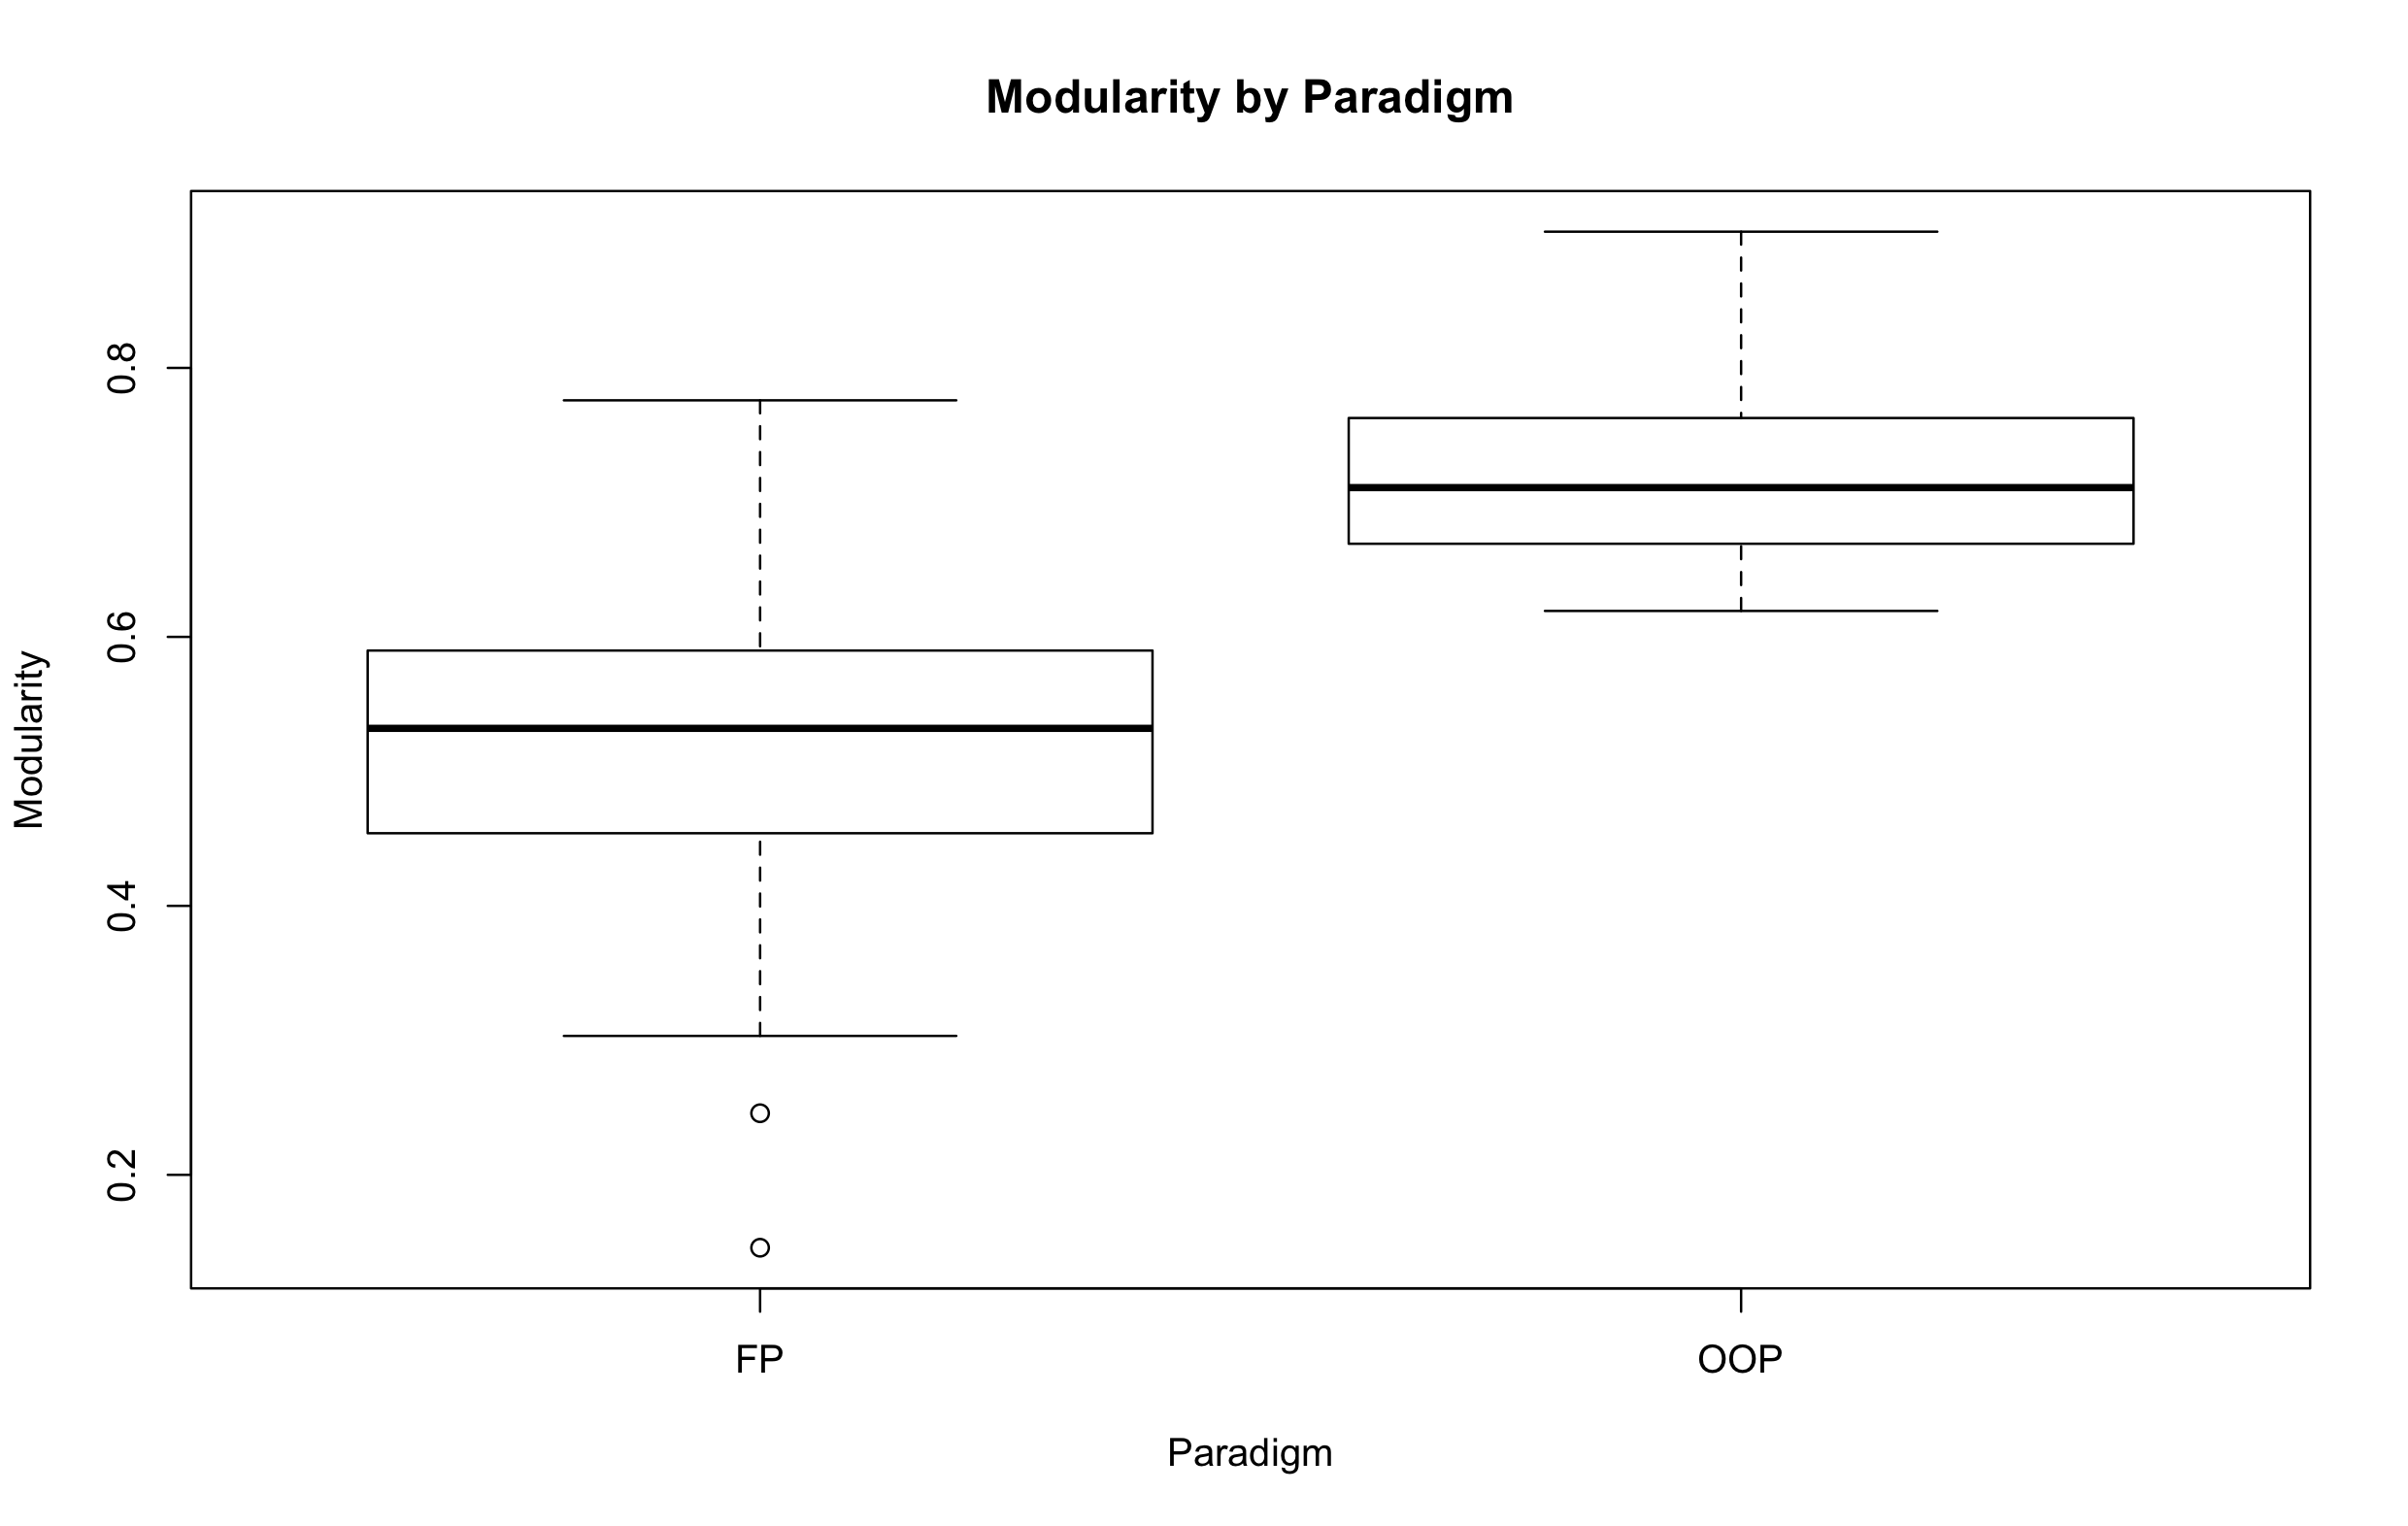
\includegraphics[width=\textwidth]{modularity_paradigm.png}
    \captionsetup{type=figure}
    \captionof{figure}{Modularity Metric Comparing both Paradigms}
    \label{fig:modularity_paradigm}
  \end{minipage}


\subsubsection{Modularity VS logarithm of lines of code}


\begin{minipage}[t]{\linewidth}
    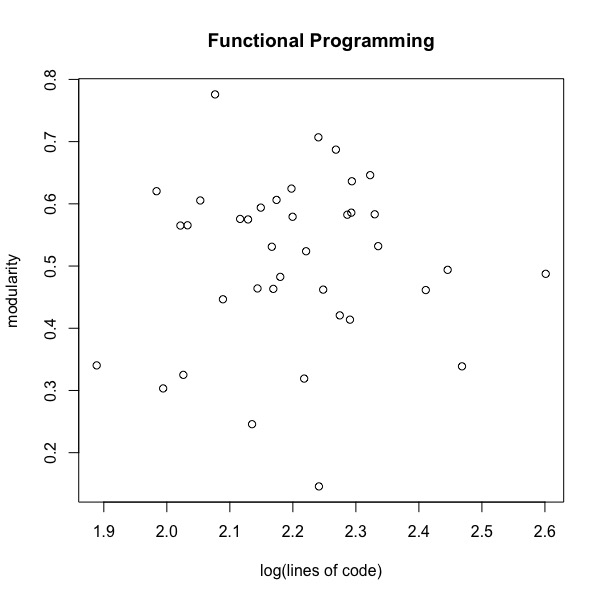
\includegraphics[width=\textwidth]{images/fp_lines_code_vs_modularity.jpeg}
    \captionsetup{type=figure}
    \captionof{figure}{Modularity VS log(Lines of Code) in FP}
    \label{fig:fp_log_lines_mod}
  \end{minipage}
  
  \begin{minipage}[t]{\linewidth}
    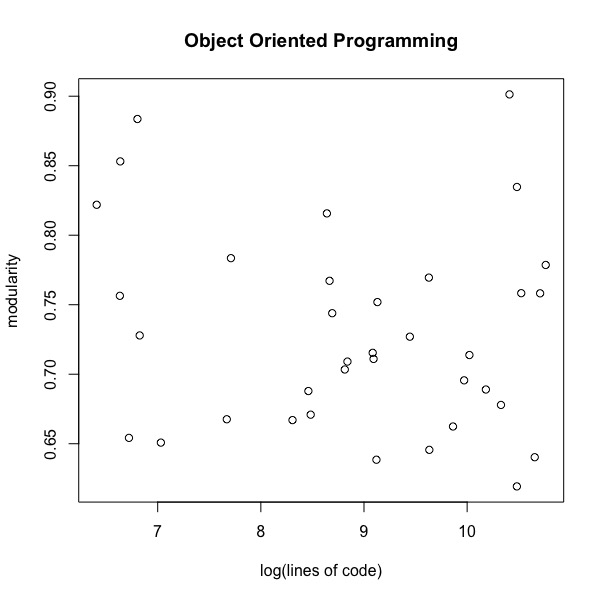
\includegraphics[width=\textwidth]{images/oop_lines_code_vs_modularity.jpeg}
    \captionsetup{type=figure}
    \captionof{figure}{Modularity VS log(Lines of Code) in OOP}
    \label{fig:oop_log_lines_mod}
  \end{minipage}

\subsubsection{Degree Distribution}
  
\begin{minipage}[t]{\linewidth}
    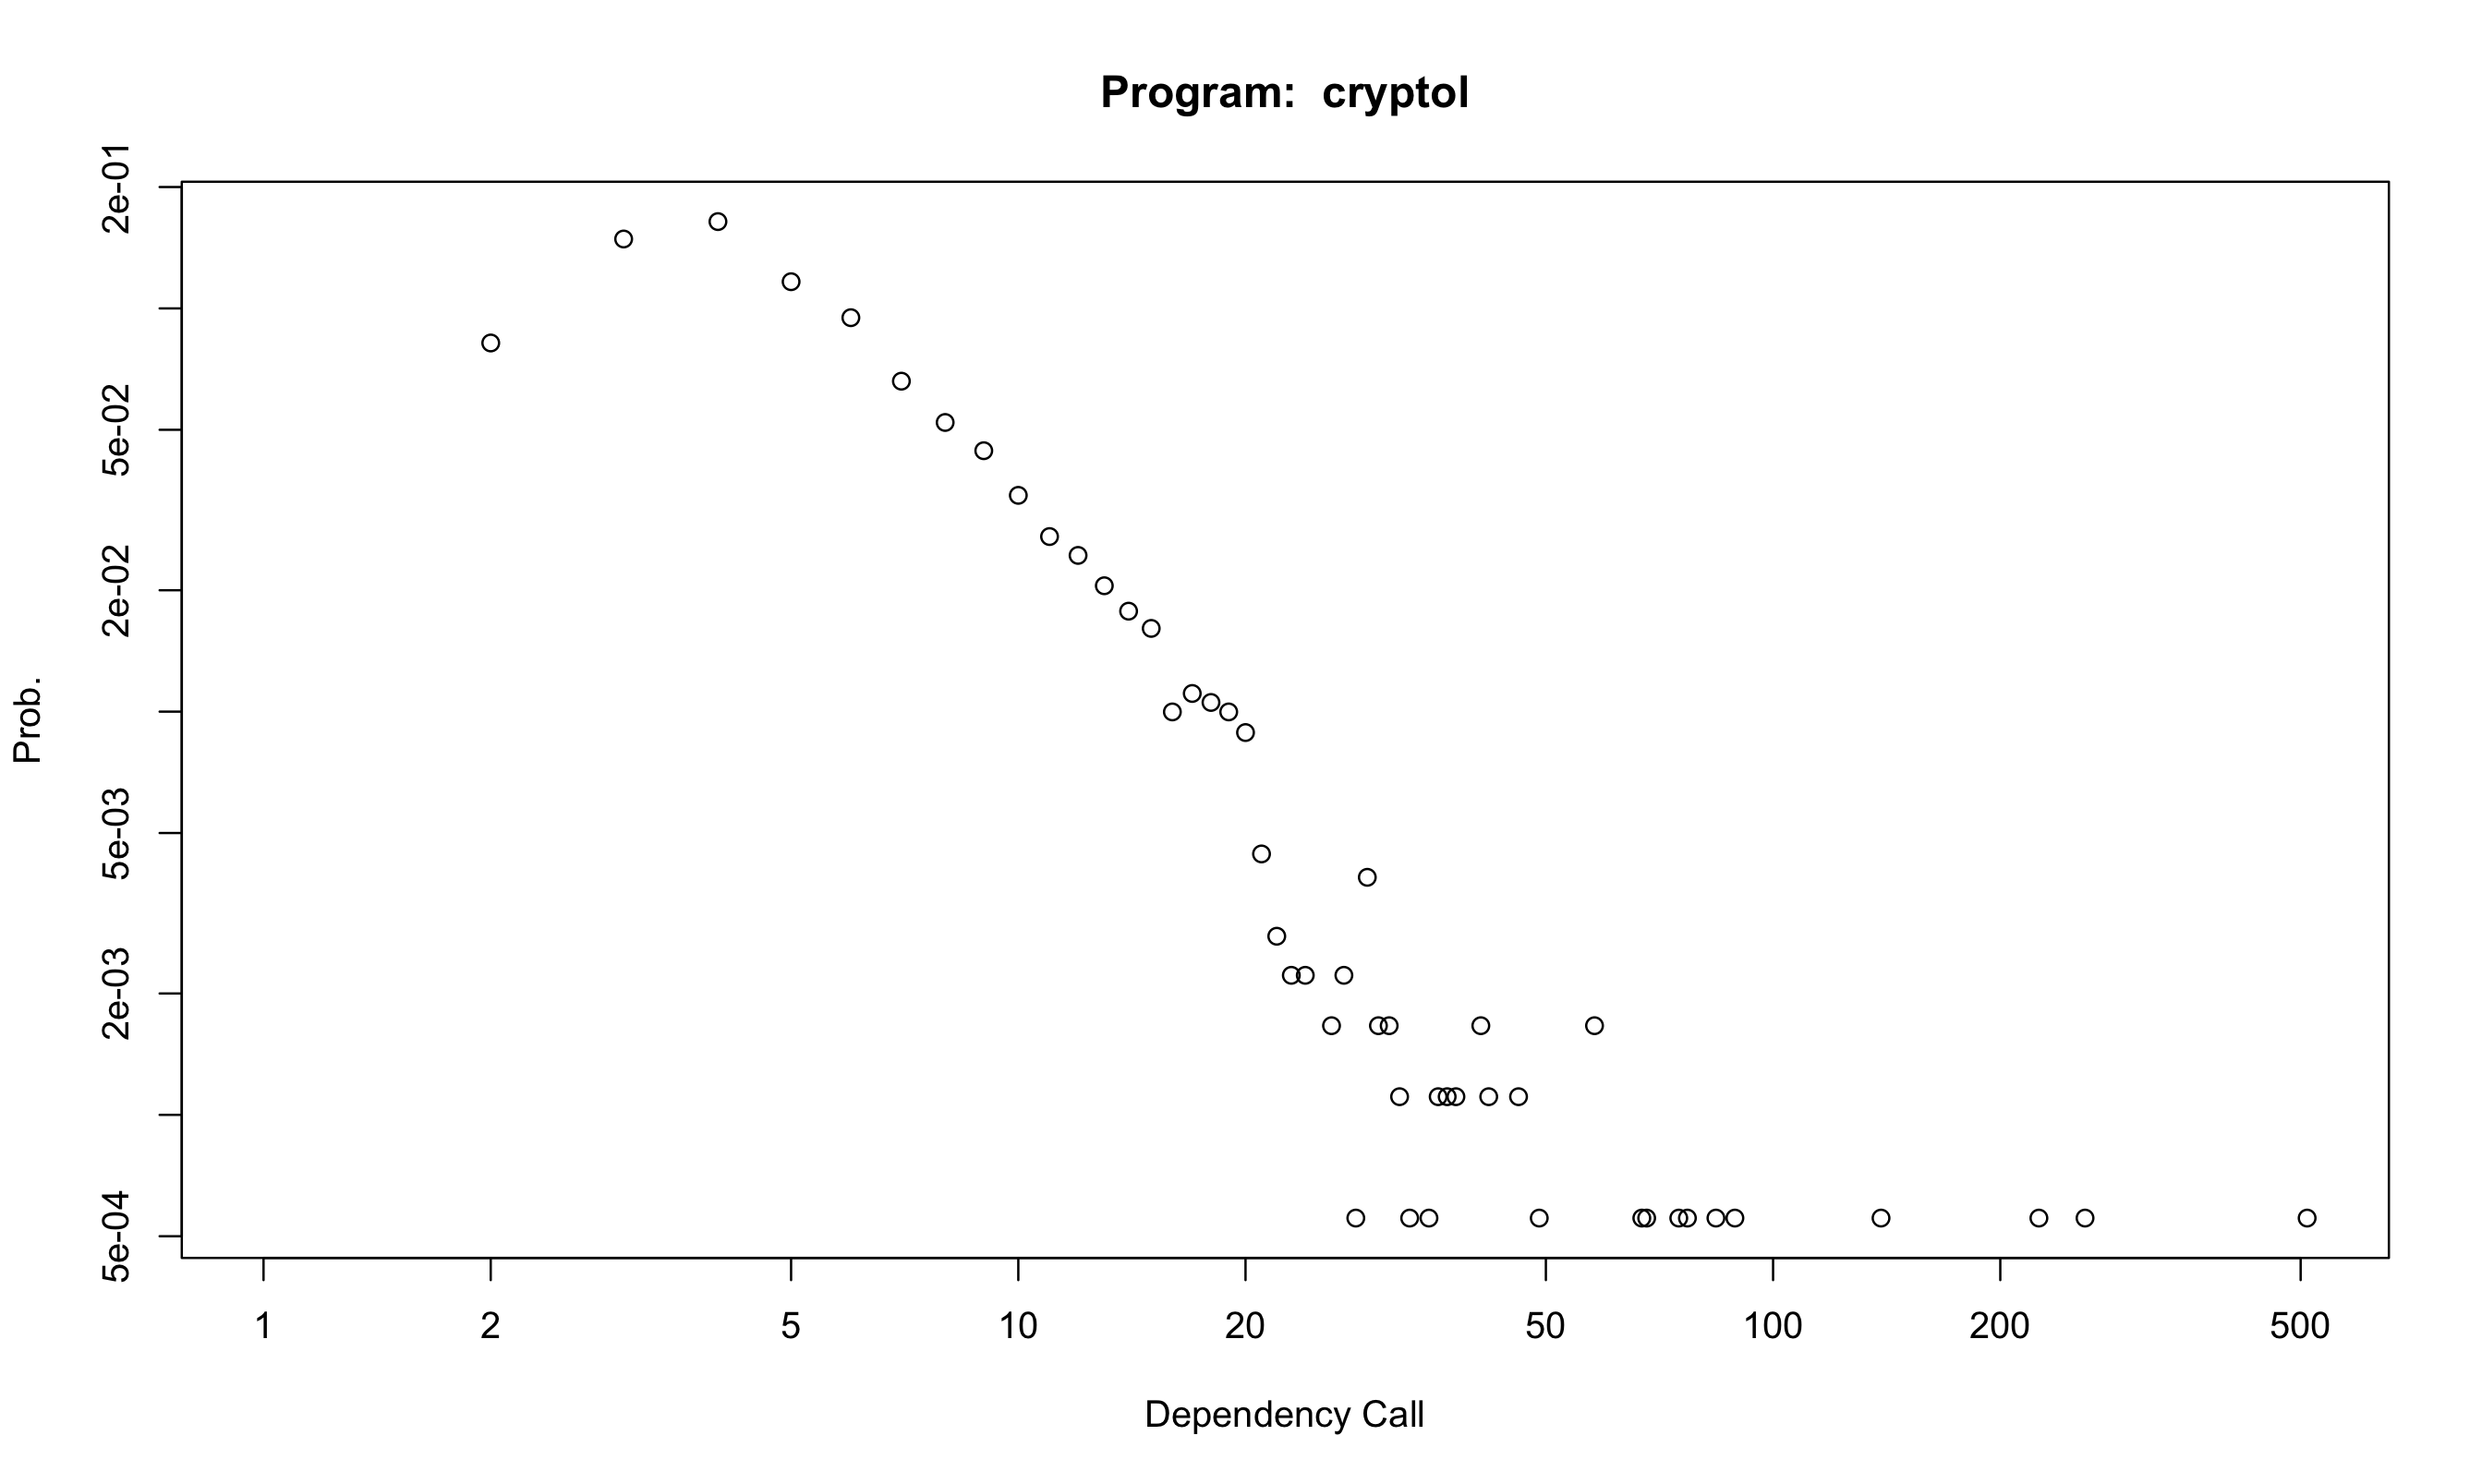
\includegraphics[width=\textwidth]{power_law_fp.png}
    \captionsetup{type=figure}
    \captionof{figure}{Example of FP Degree Distribution}
    \label{fig:power_law_fp}
  \end{minipage}

  \begin{minipage}[t]{\linewidth}
    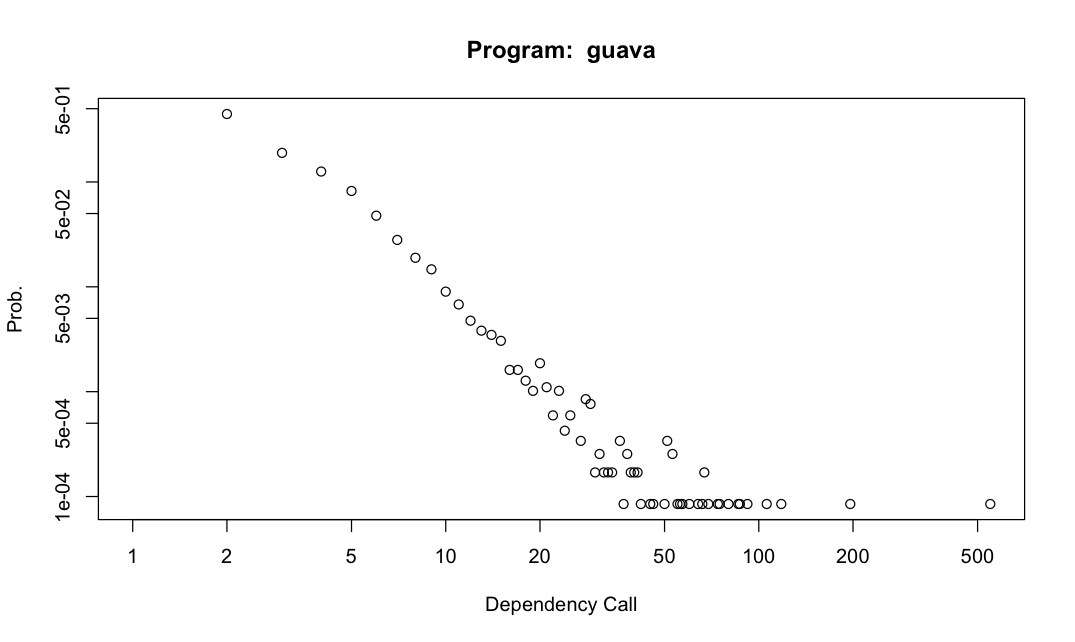
\includegraphics[width=\textwidth]{power_law_oop.png}
    \captionsetup{type=figure}
    \captionof{figure}{Example of OOP Degree Distribution}
    \label{fig:power_law_oop}
  \end{minipage}




\section{Discussion and Analysis}

Here we are going to discuss the results obtained in our experiments.

\subsection{Hypothesis 1}

We have provided the framework to analyze a new program passed as input. We think that this is a good training set to fit our framework. Now any program passed as input should be categorized as bad-designed-software or good-designed-software if its metrics fall inside the first and third quartile of all (or the majority) metrics computed.

\subsection{Hypothesis 2}

As we can see in Figure 1 we can accept our Hypothesis. This is something expected as OOP paradigm has this modularity philosophy (classes, objects, setters, getters,...) in its core design principles. 

\subsection{Hypothesis 3}

As we can see in Figure 2 and 3 we have to reject our Hypothesis as we can't see that there exist a clear relationship between this 2 variables. It is enough to check visually the images to make this statement. \\ \\ Our hypothesis was based on the intuition that when a program becomes bigger in terms of lines of code it has to be more modularized in order to be able to maintain it as developers.

\subsection{Hypothesis 4}

This hypothesis can also be accepted. We used a model fitting technique to see that a power-law like function is the most suited to fit this model (giving the lower AIC).  \\

This was also expected because the vast majority of functions/packages have just few outside calls.



\section{Conclusions}

We started this project inspired by XXXX where they used a refined modularity metric in order to asses the quality of Low Coupling and High cohesion. \\
We have focused our study not only in this mentioned aspect but also in :

\begin{itemize}
  \item Trying to see other typical properties that good-design-software has, as power-law-like degree distribution in its Call dependency graph.
  \item Capturing differences between different software paradigms in terms of modularity.
  \item Trying to find some relationship between the 2 metrics of a software program (lines of code and modularity).
\end{itemize}\\

In order to do this project, a dataset of programs was needed and the collection of it it was the most tedious aspect in the project. This collection has been made by hand in different online repositories mentioned in the References. \\
For instance in the case of Java programs, to generate the Call dependency grah, a jar file was needed and it is not common to find them online.\\ An alternative was downloading the source files a packaging them but this is not a sustainable method if you want to have a considerable amount of observations in your dataset as a lot of problems usually appear during compilation and packaging to should be solved meticulously. \\ Possibly a good idea could be develop a tool that can generate the CDG from the source files.

This is the reason why other hypothesis that were proposed at the fist moment as finding the relationship between modularity and number of code refactors in the code (counted with number of commits) or finding the relationship between modularity and number of contributors in a project were discarded (Github provides this 2 metrics for each project, i.e, number of commits and number of contributors).
\newpage







\bibliographystyle{alpha}
\bibliography{Report}

\appendix
\section{Organization}\label{apx:sec:org:1}

\begin{itemize}
    \item \textbf{code}: Under this folder you are going to find \textit{R Scripts} code for conducting this analysis.
    \item \textbf{fp\_graphs}: \textit{DOT} files that contains the Dependency Graph Representation of each \acrlong{fp} Program
    \item \textbf{oop\_graphs}: \textit{DOT} files that contains the Dependency Graph Representation of each \acrlong{oop} Program
    \item \textbf{report}: This report in Latex and PDF format.
\end{itemize}

\section{Programs Details - Line of Codes}\label{apx:sec:loc}
\subsection{FP Programs}
\begin{longtable}[H]{l r}
    \caption{FP Analyzed Programs}\label{table:ax_fp_prog_1}\\
        Program & LoC \\
        \hline            
        \endhead
        aeson & 6948 \\
        amazonka & 715531 \\
        async & 743 \\
        attoparsec & 4718 \\
        beam & 20151 \\
        cabal & 102525 \\
        co-log & 1436 \\
        conduit & 12963 \\
        containers & 19556 \\
        criterion & 2421 \\
        cryptol & 30740 \\
        cryptonite & 18763 \\
        dhall & 29058 \\
        free & 4472 \\
        fused-effects & 4145 \\
        ghcid & 1664 \\
        haskoin & 12066 \\
        hedgehog & 8277 \\
        helm & 2071 \\
        hlint & 6306 \\
        lens & 16691 \\
        liquid & 133740 \\
        megaparsec & 8144 \\
        mios & 6178 \\
        mtl & 932 \\
        optparse & 3220 \\
        pandoc & 69179 \\
        pipes & 1969 \\
        postgresql & 6596 \\
        protolude & 1901 \\
        quickcheck & 5077 \\
        reflex & 10062 \\
        relude & 2913 \\
        servant & 15725 \\
        snap & 5310 \\
        stm & 1550 \\
        summoner & 4025 \\
        text & 9783 \\
        vector & 12166 \\
        yesod & 19971 \\
        PRIVATE PROGRAM & 26975
\end{longtable}

\subsection{OOP Analytzed Programs}
\begin{longtable}[H]{l r}
    \caption{OOP Analyzed Programs}\label{table:ax_oop_prog_1}\\
        Program & LoC \\
        \hline            
        \endhead
        akka-actor\_2.10-2.3.9 & 35702 \\
        commons-cli-1.4 & 830 \\
        commons-codec-1.10 & 2231 \\
        commons-csv-1.8 & 607 \\
        commons-email-1.4 & 760 \\
        disruptor-3.4.2 & 1131 \\
        ftpserver-core-1.0.6 & 4052 \\
        grpc-core-1.34.1 & 9142 \\
        guava-28.1-jre & 37216 \\
        hbase-client-2.4.0 & 33209 \\
        hsqldb-2.4.1 & 30578 \\
        jackson-databind-2.12.0 & 22516 \\
        javax.servlet-api-4.0.1 & 901 \\
        jedis-3.4.1 & 12640 \\
        jersey-core-1.19.4 & 5656 \\
        jetty-7.0.0.pre5 & 6727 \\
        joda-time-2.10.6 & 8891 \\
        jsch-0.1.54 & 4833 \\
        jsoup-1.13.1 & 5955 \\
        junit-4.13.1 & 5803 \\
        mail-1.4.7 & 8817 \\
        mariadb-java-client-2.7.1 & 9229 \\
        mongo-java-driver-3.12.7 & 35676 \\
        mx4j-3.0.2 & 6902 \\
        org.eclipse.jgit & 42417 \\
        pdfbox-2.0.22 & 26413 \\
        poi-4.1.2 & 44691 \\
        postgresql-42.2.18 & 15199 \\
        resteasy-jaxrs-3.14.0.Final & 15267 \\
        runtime-3.10.0-v20140318-2214 & 921 \\
        slf4j-api-1.7.30 & 763 \\
        spring-security-core-5.4.2 & 4726 \\
        spring-web-5.3.2 & 21393 \\
        tomcat-embed-core-10.0.0 & 47185 \\
        zookeeper-3.6.2 & 19207 \\
        PRIVATE PROGRAM & 2143
\end{longtable}

\end{document}

